\begin{figure}[h!]
  \centering
    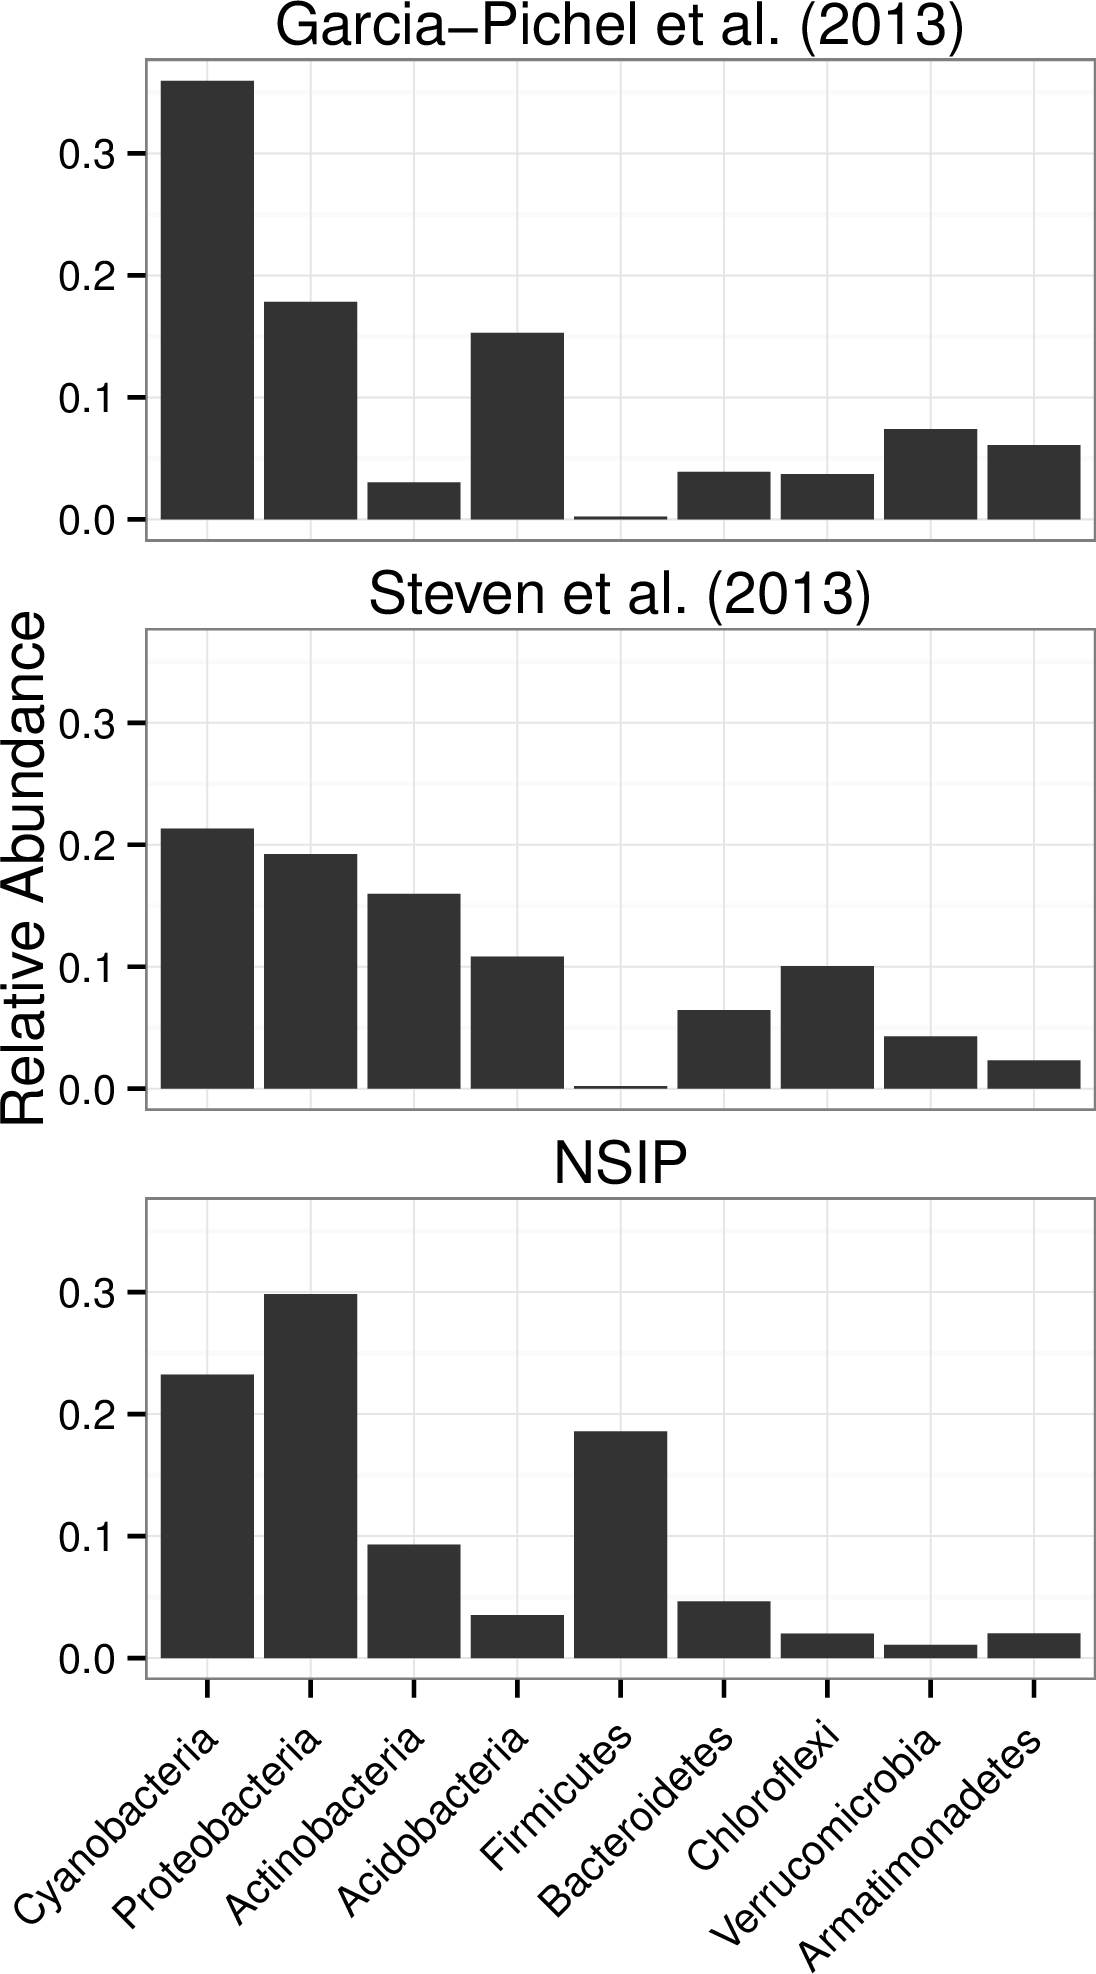
\includegraphics[width=1.0\textwidth]{figures/study_phylum_dist/study_phylum_dist.png}
  \caption{Distribution of sequences into top 9 phyla (phyla ranked by sum of all sequence annotations).}
  \label{fig:study_phy_dist}
\end{figure}

\begin{figure}[h!]
  \centering
  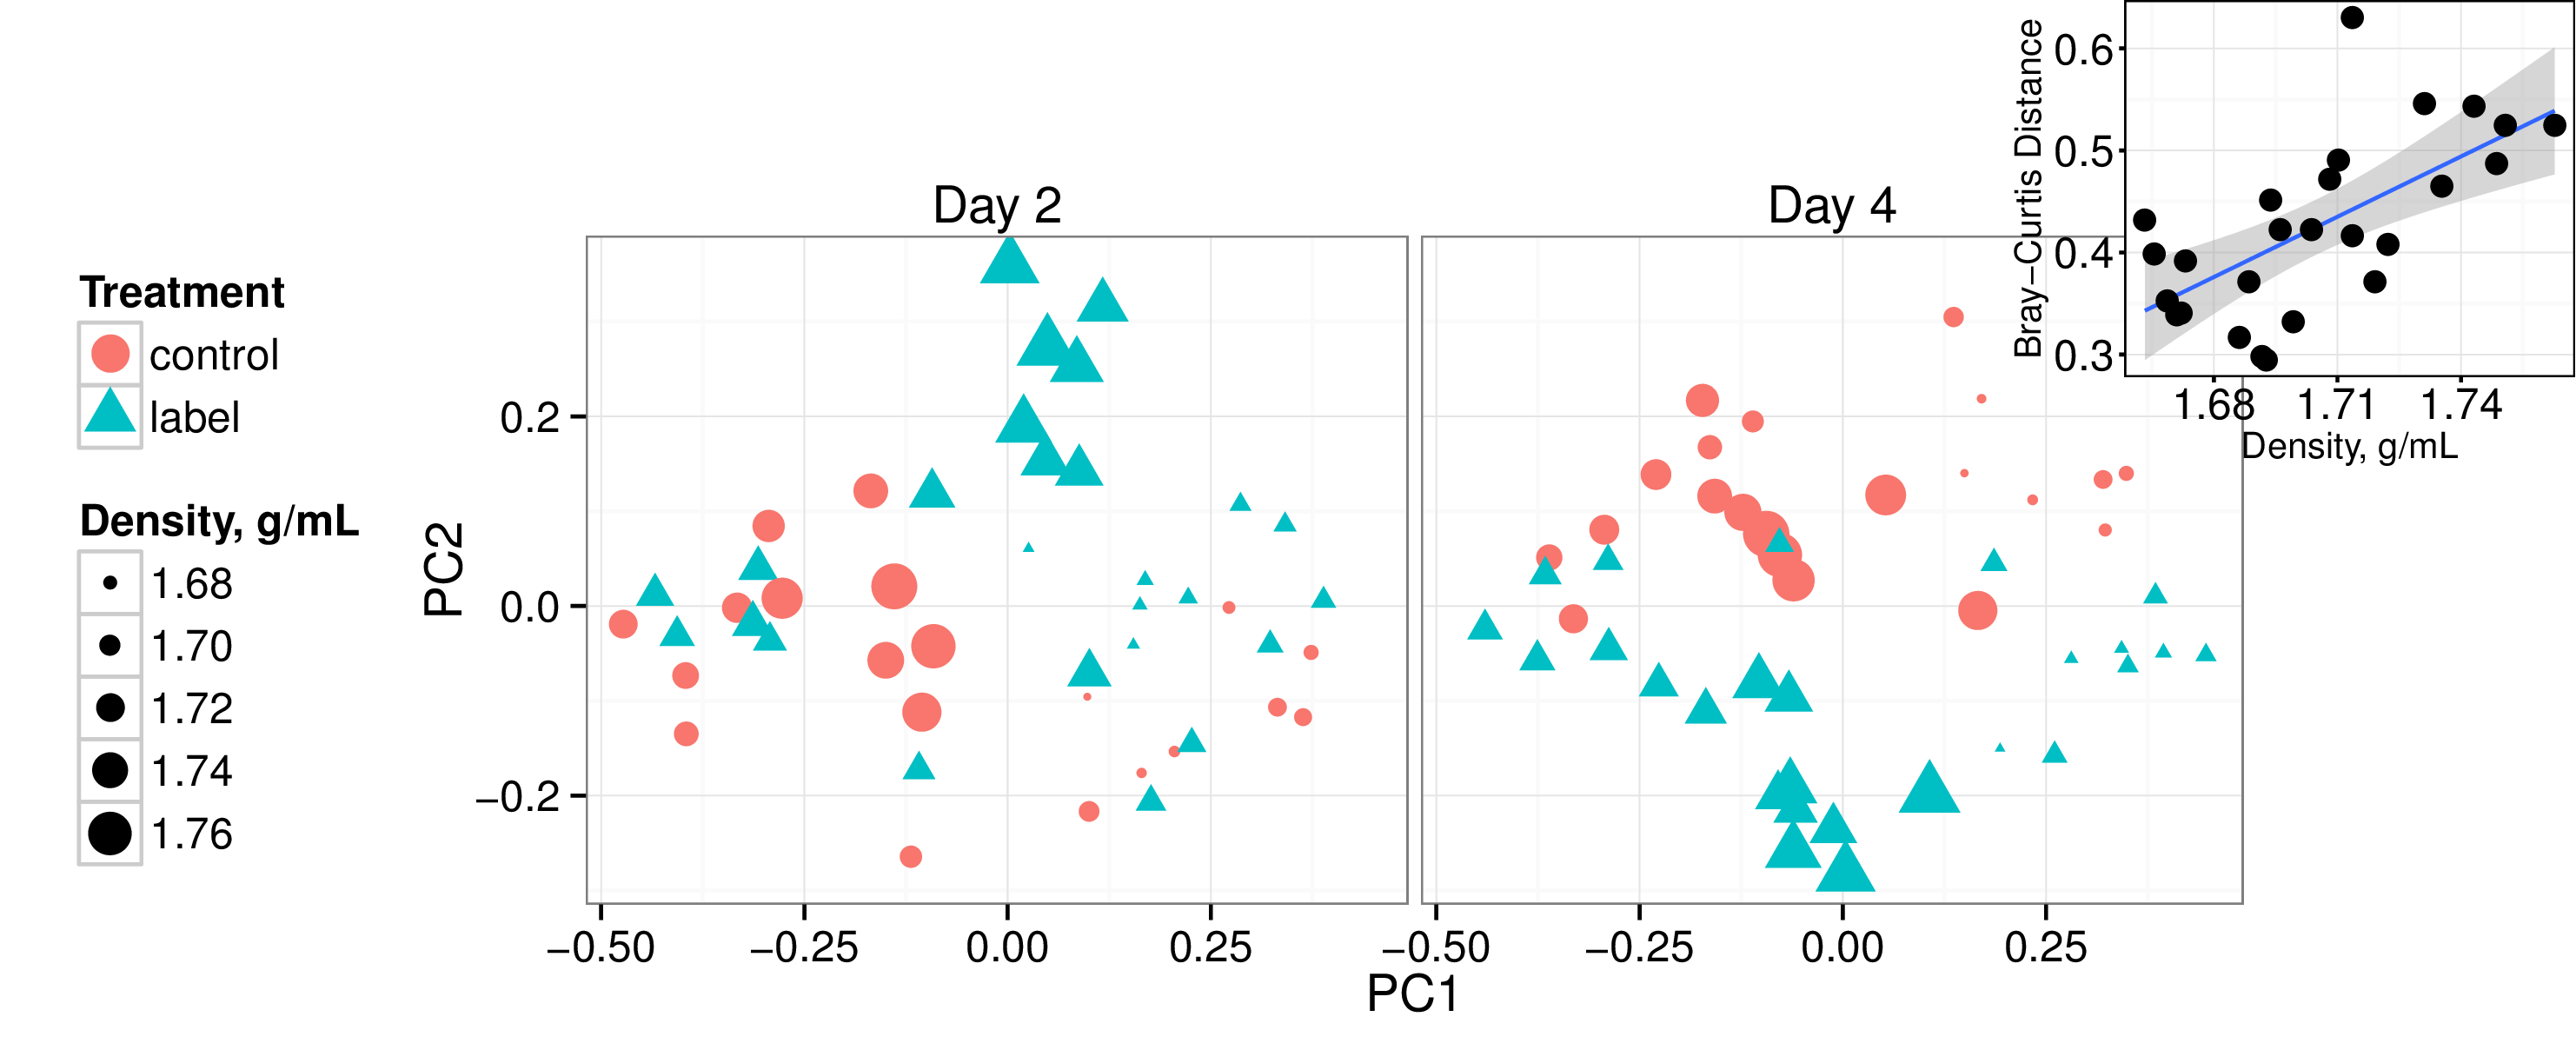
\includegraphics[width=1.0\textwidth]{figures/ordination_all_day_facet/ordination_day_facet_w_inset.png}
  \caption{Ordination of Bray-Curtis sample pairwise distances for each incubation time. Point area is proportional to the density of the CsCl gradient fraction for each sequence library, and color reflects control (red) or labeled (blue) treatment. Inset shows Bray-Curtis distances for paired control versus labeled CsCl gradient fractions (i.e. fractions from the same incubation day and same density) against the density of the pair (p-value: 0.000517, r$^{2}$: 0.332).}
  \label{fig:ordination}
\end{figure}

\begin{figure}[h!]
  \centering
    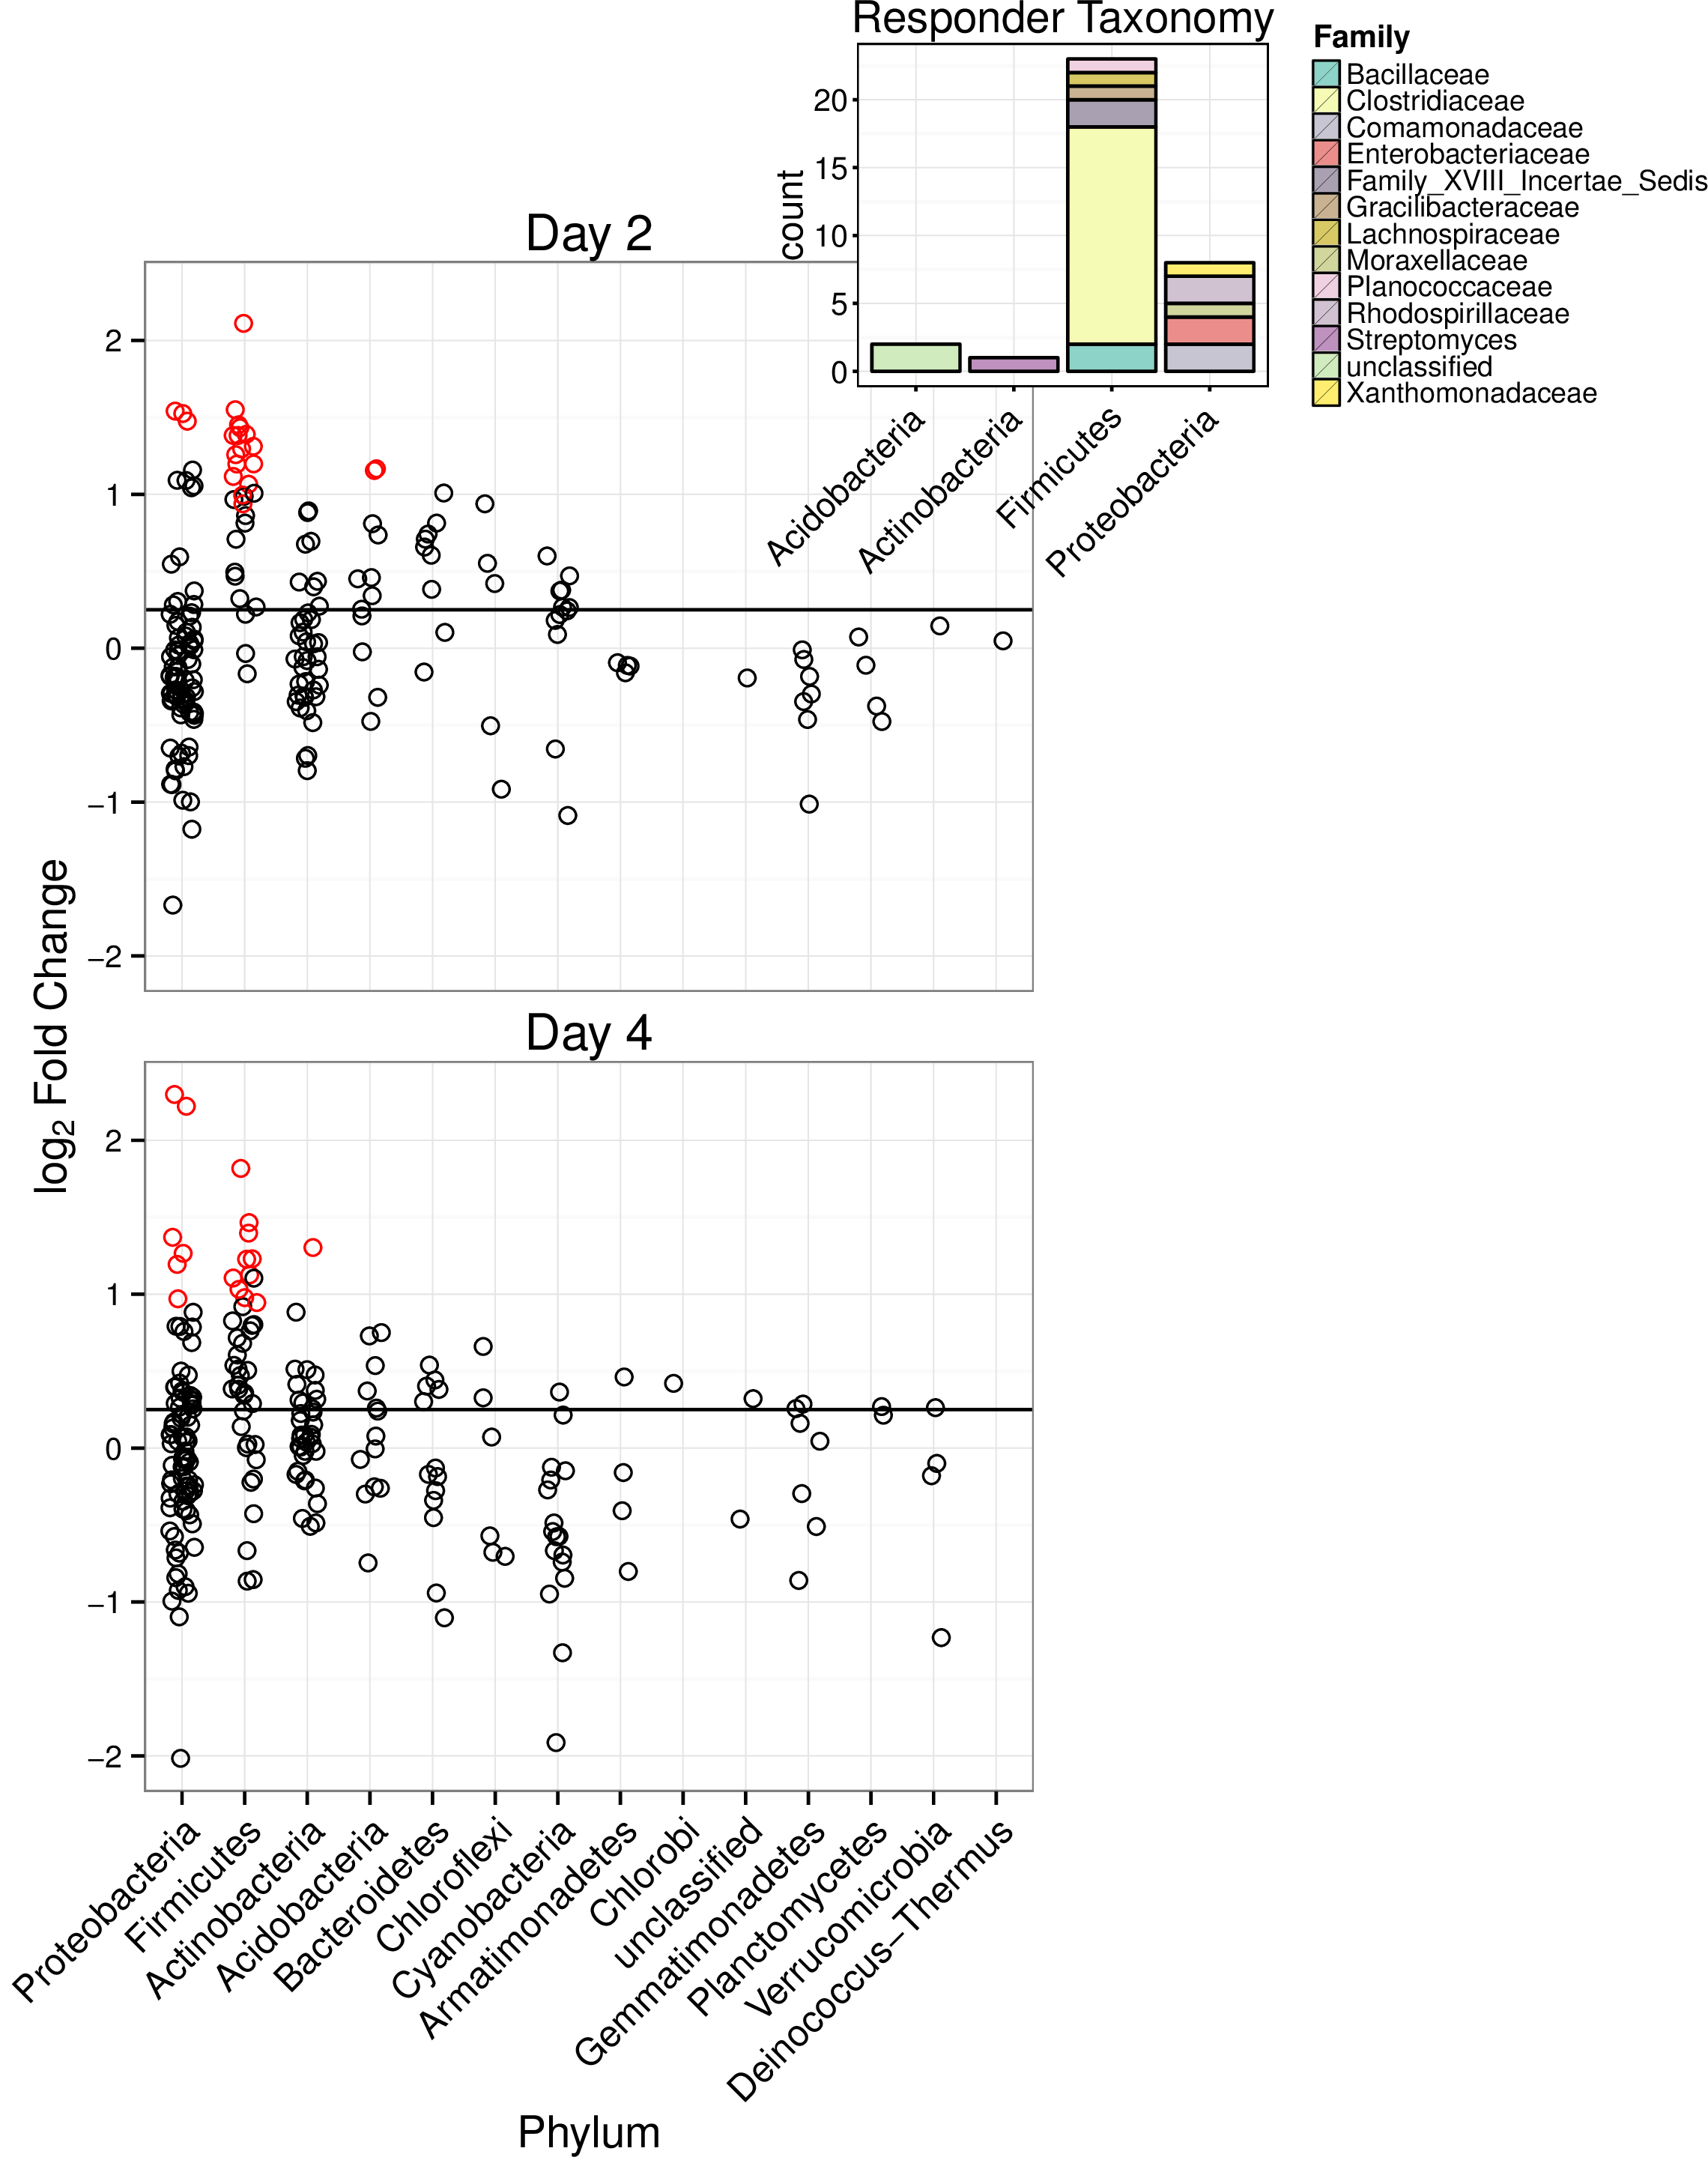
\includegraphics[width=1.0\textwidth]{figures/l2fc1/l2fc_stacked_w_inset.png}
  \caption{Moderated log$_{2}$ of proportion mean ratios for labeled versus control gradients (heavy fractions only, densities >1.725 g/mL). All OTUs found in at least 62.5\% of heavy fractions at a specific incubation day are shown. Red color denotes a proportion mean ratio that has a corresponding adjusted p-value below a false discovery rate of 10\% (the null model is that the proportion mean is ratio is below 0.25). The horizontal line is the proportion mean threshold for the null model, 0.25. The inset figure summarizes the taxonomy of OTUs that with proportion mean ratio p-vaules under 0.10 for at least one time point.}
  \label{fig:l2fc}
\end{figure}

\begin{figure}[h!]
  \centering
    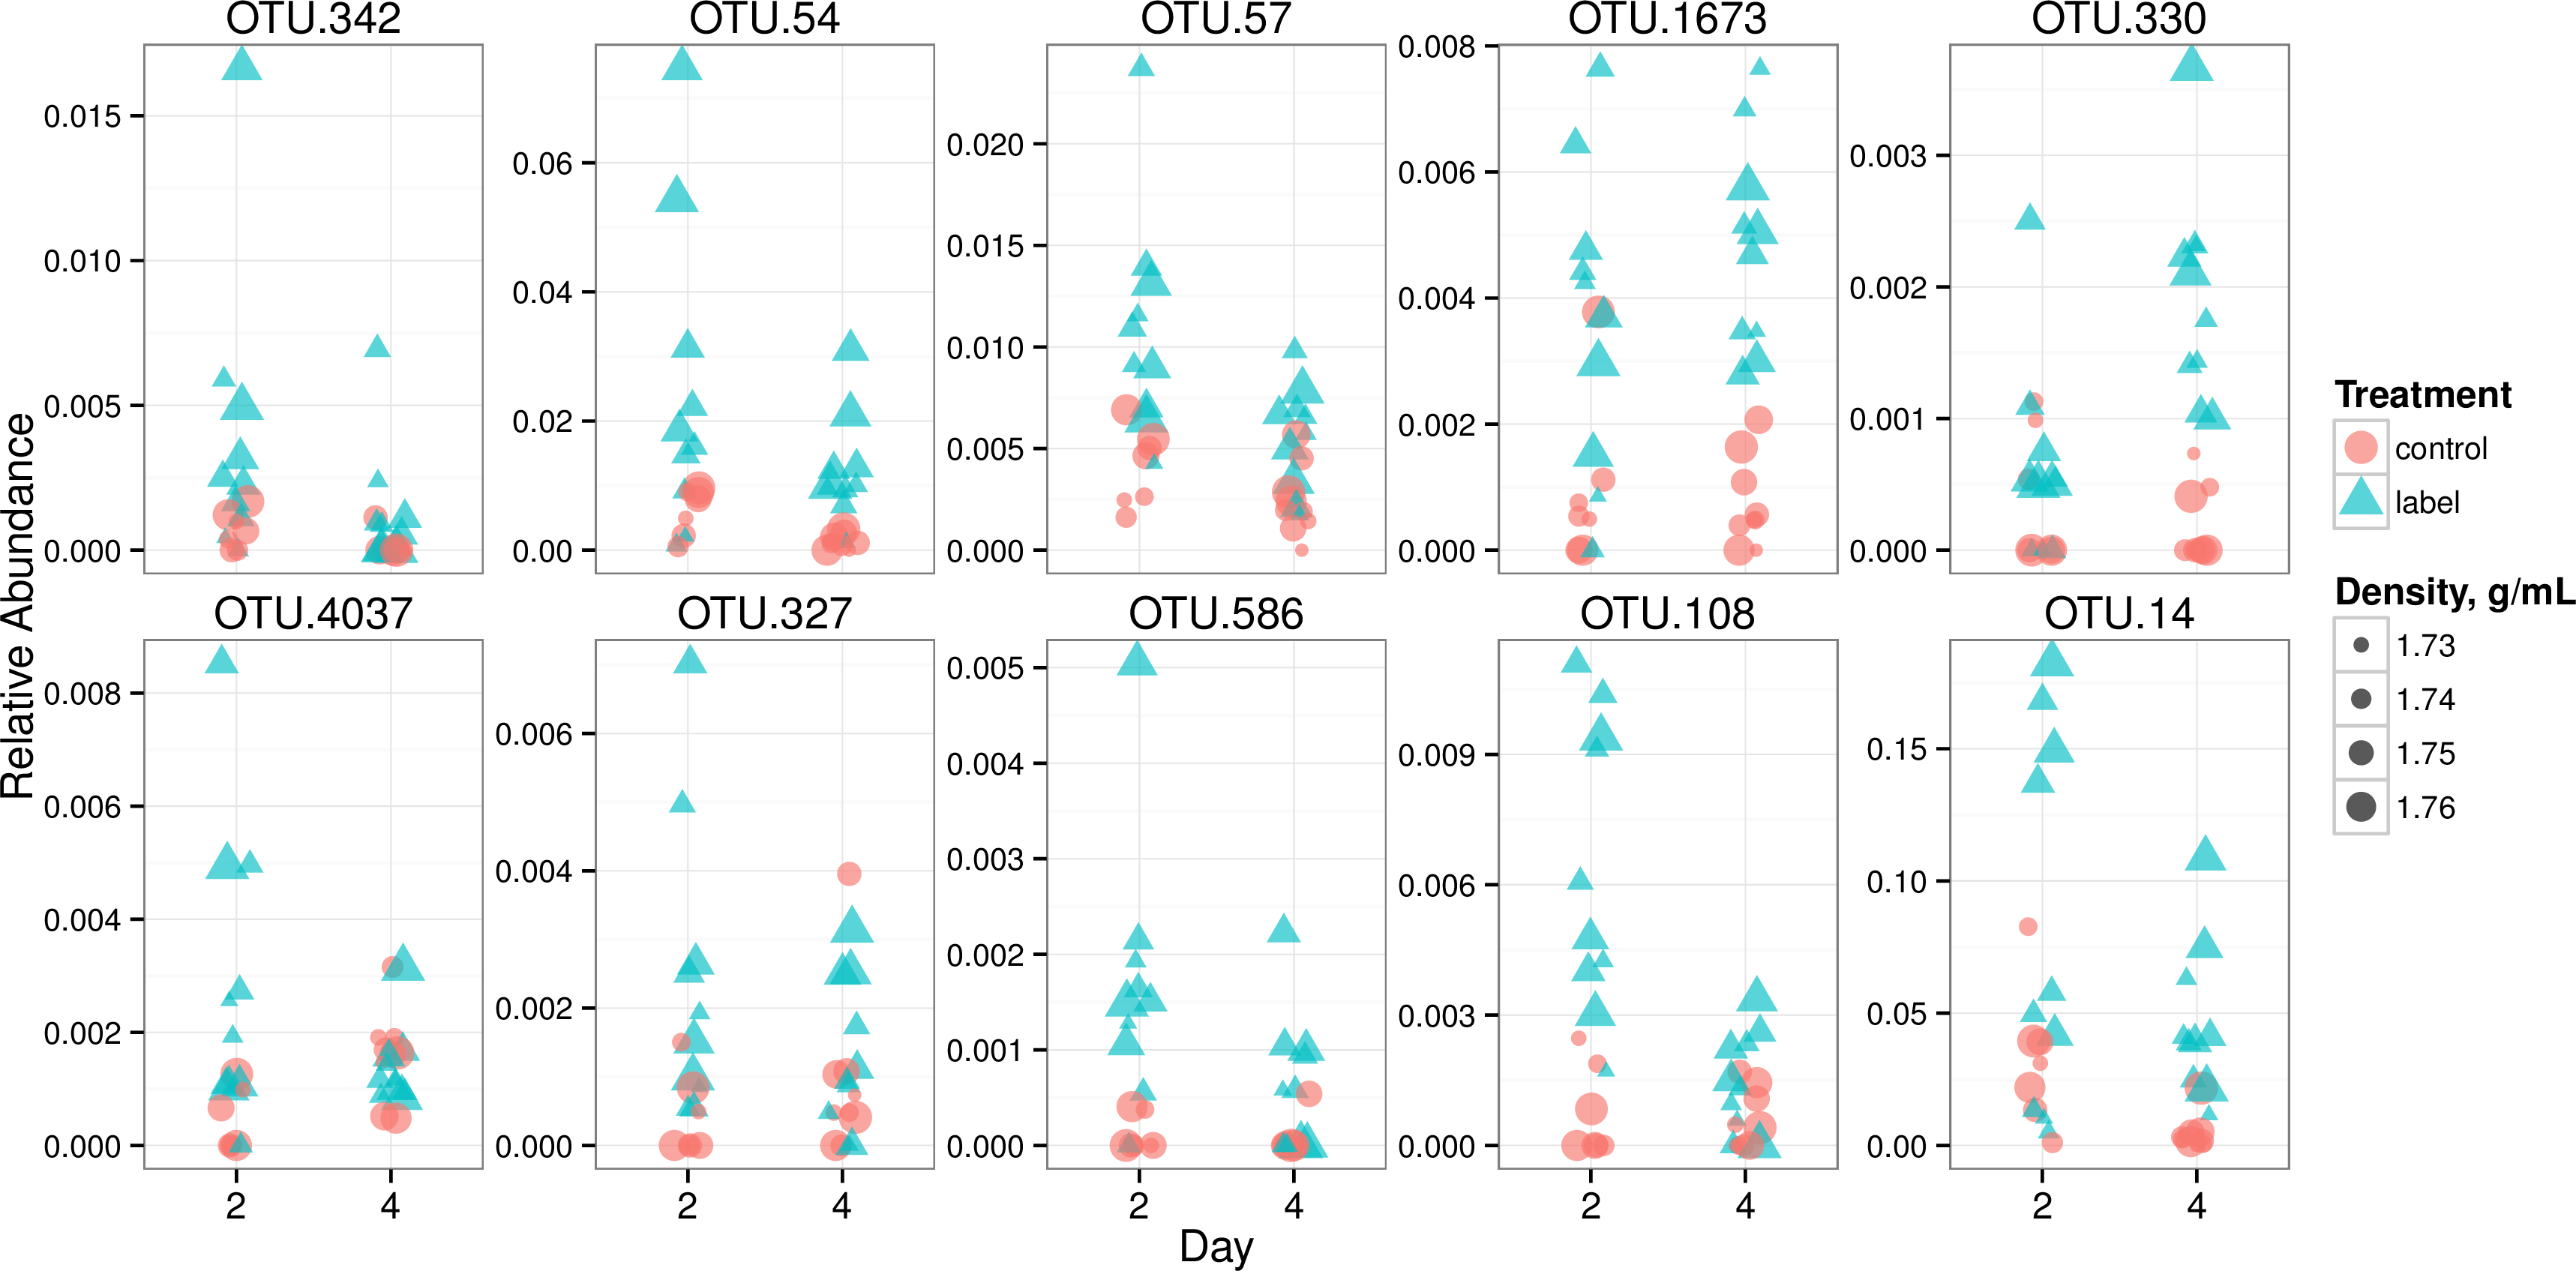
\includegraphics[width=1.0\textwidth]{figures/scatter_heavy_topN2/scatter_heavy_topN.png}
  \caption{Relative abundance values in heavy fractions (density greater or equal to 1.725 g/mL) for the top 10 $^{15}$N "responders" (putative diazotrophs, see results for selection criteria of top 10) at each incubation day. See Table X for BLAST results of top 10 responders against the LTP database (release 115). Point area is proportional to CsCl gradient fraction density, and color signifies control (red) or labeled (blue) treatment.}
  \label{fig:scatter_heavy}
\end{figure}

\begin{figure}[h!]
  \centering
    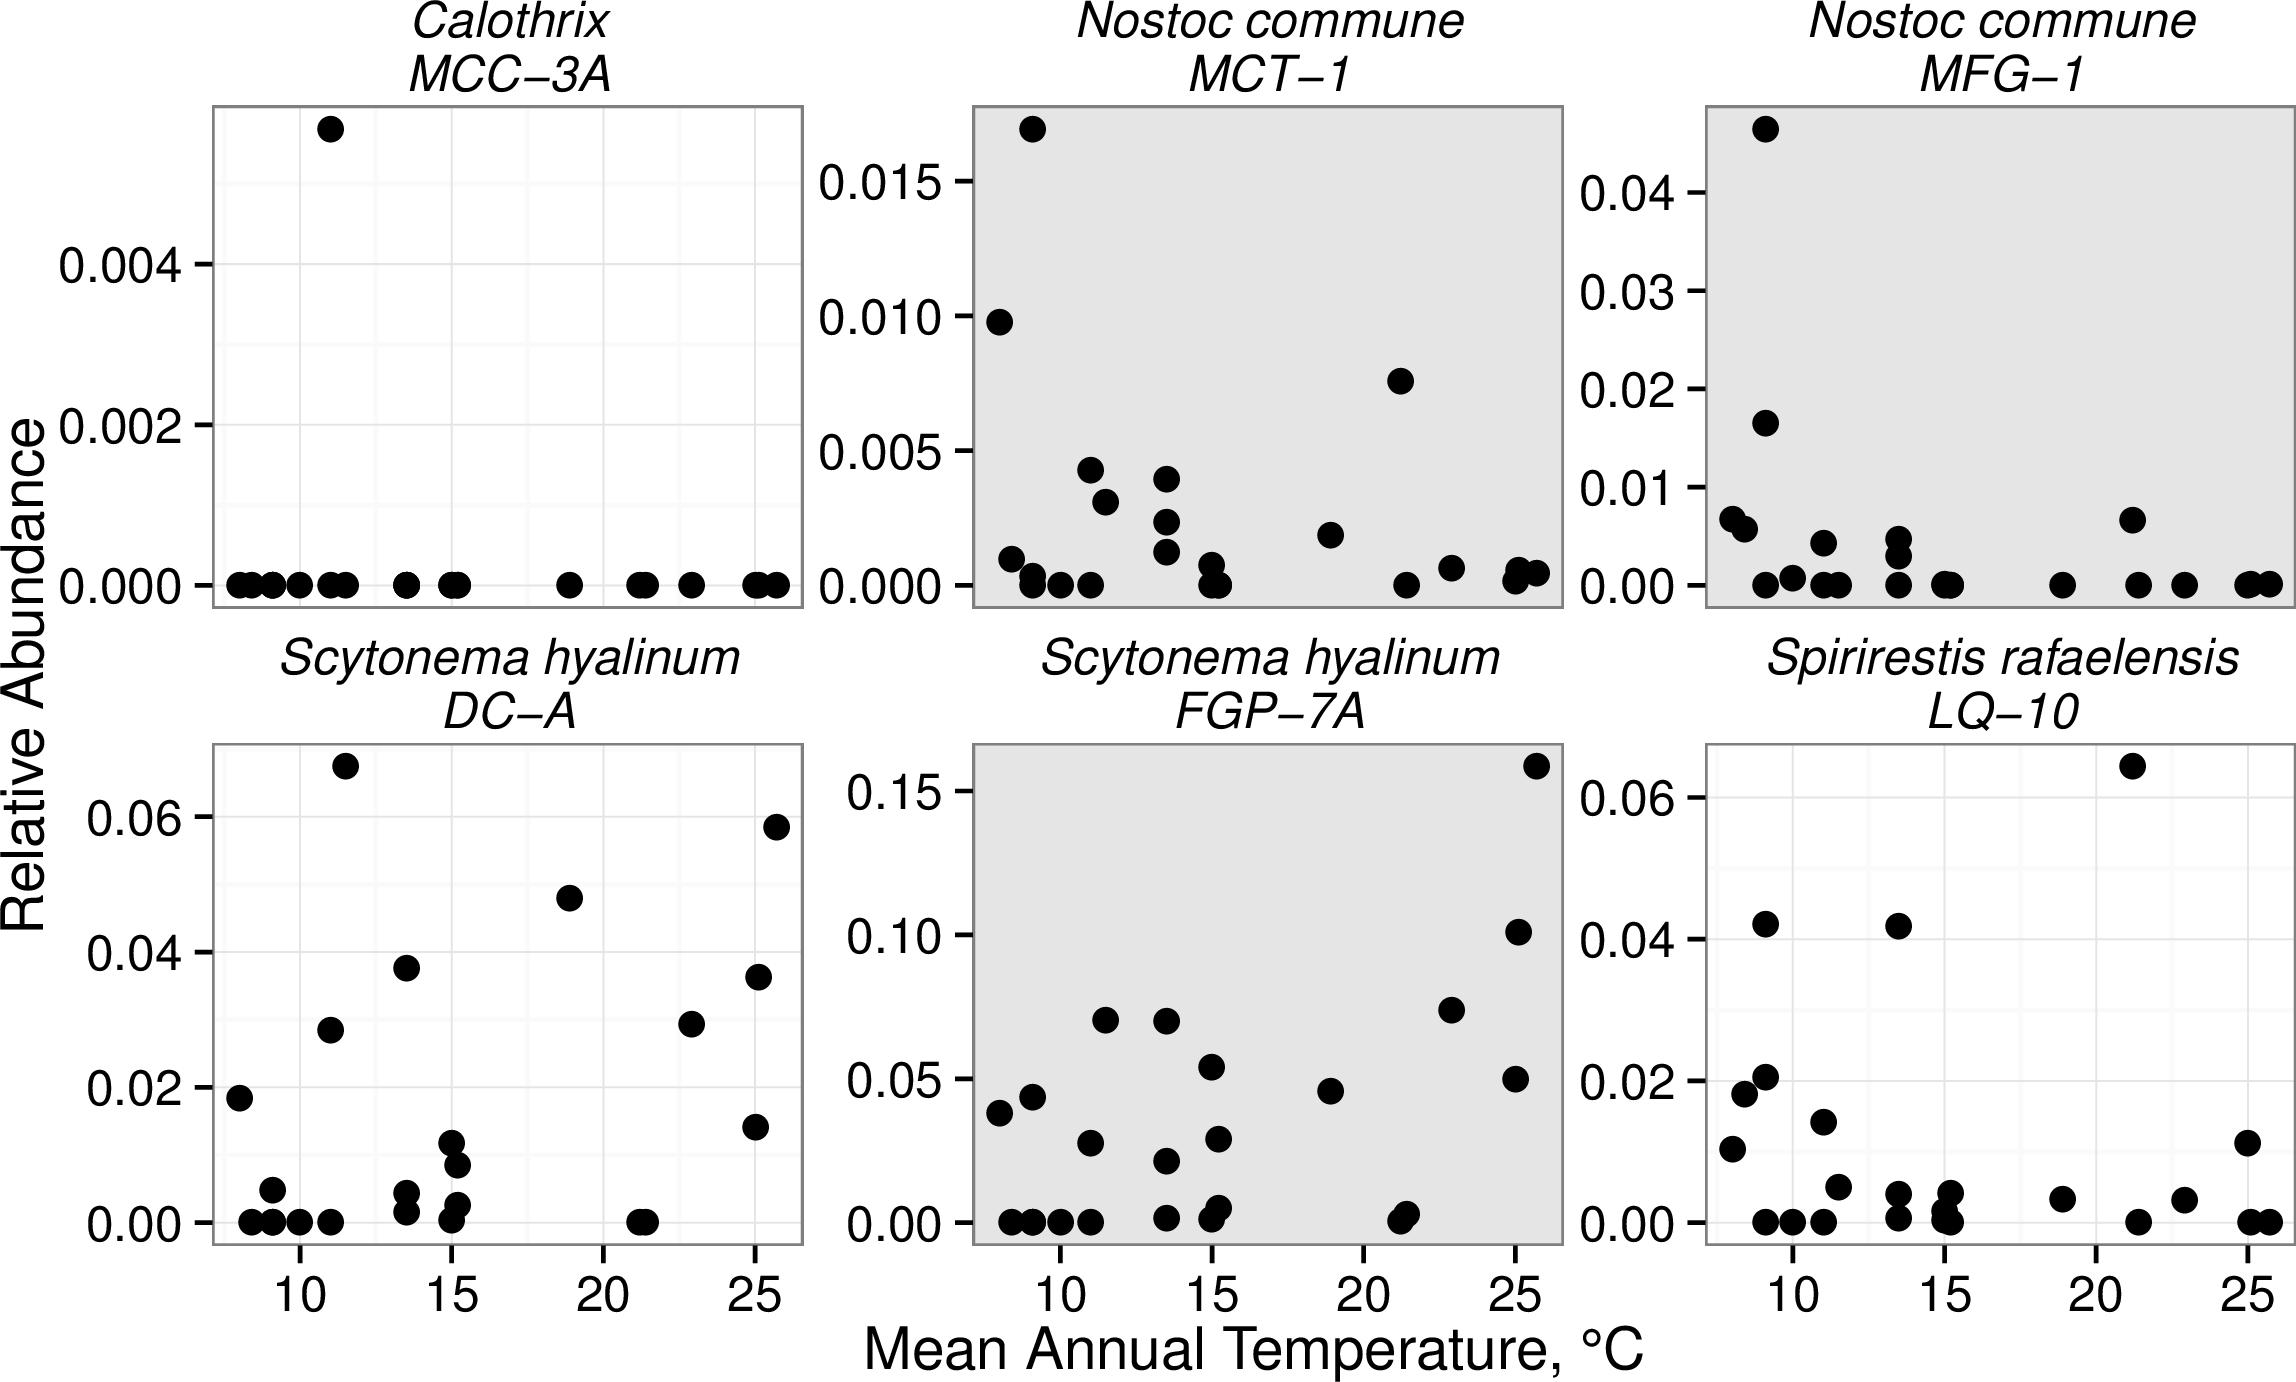
\includegraphics[width=1.0\textwidth]{figures/het_cyano_temp/het_cyano_temp.png}
  \caption{Relative abundance of selected heterocystous cyanobacterial OTUs with centroids from sequences described in \citet{Yeager} (see methods for selection criteria) in \citet{Steven_2013} data set.}
  \label{fig:het_temp}
\end{figure}

\begin{figure}[h!]
  \centering
    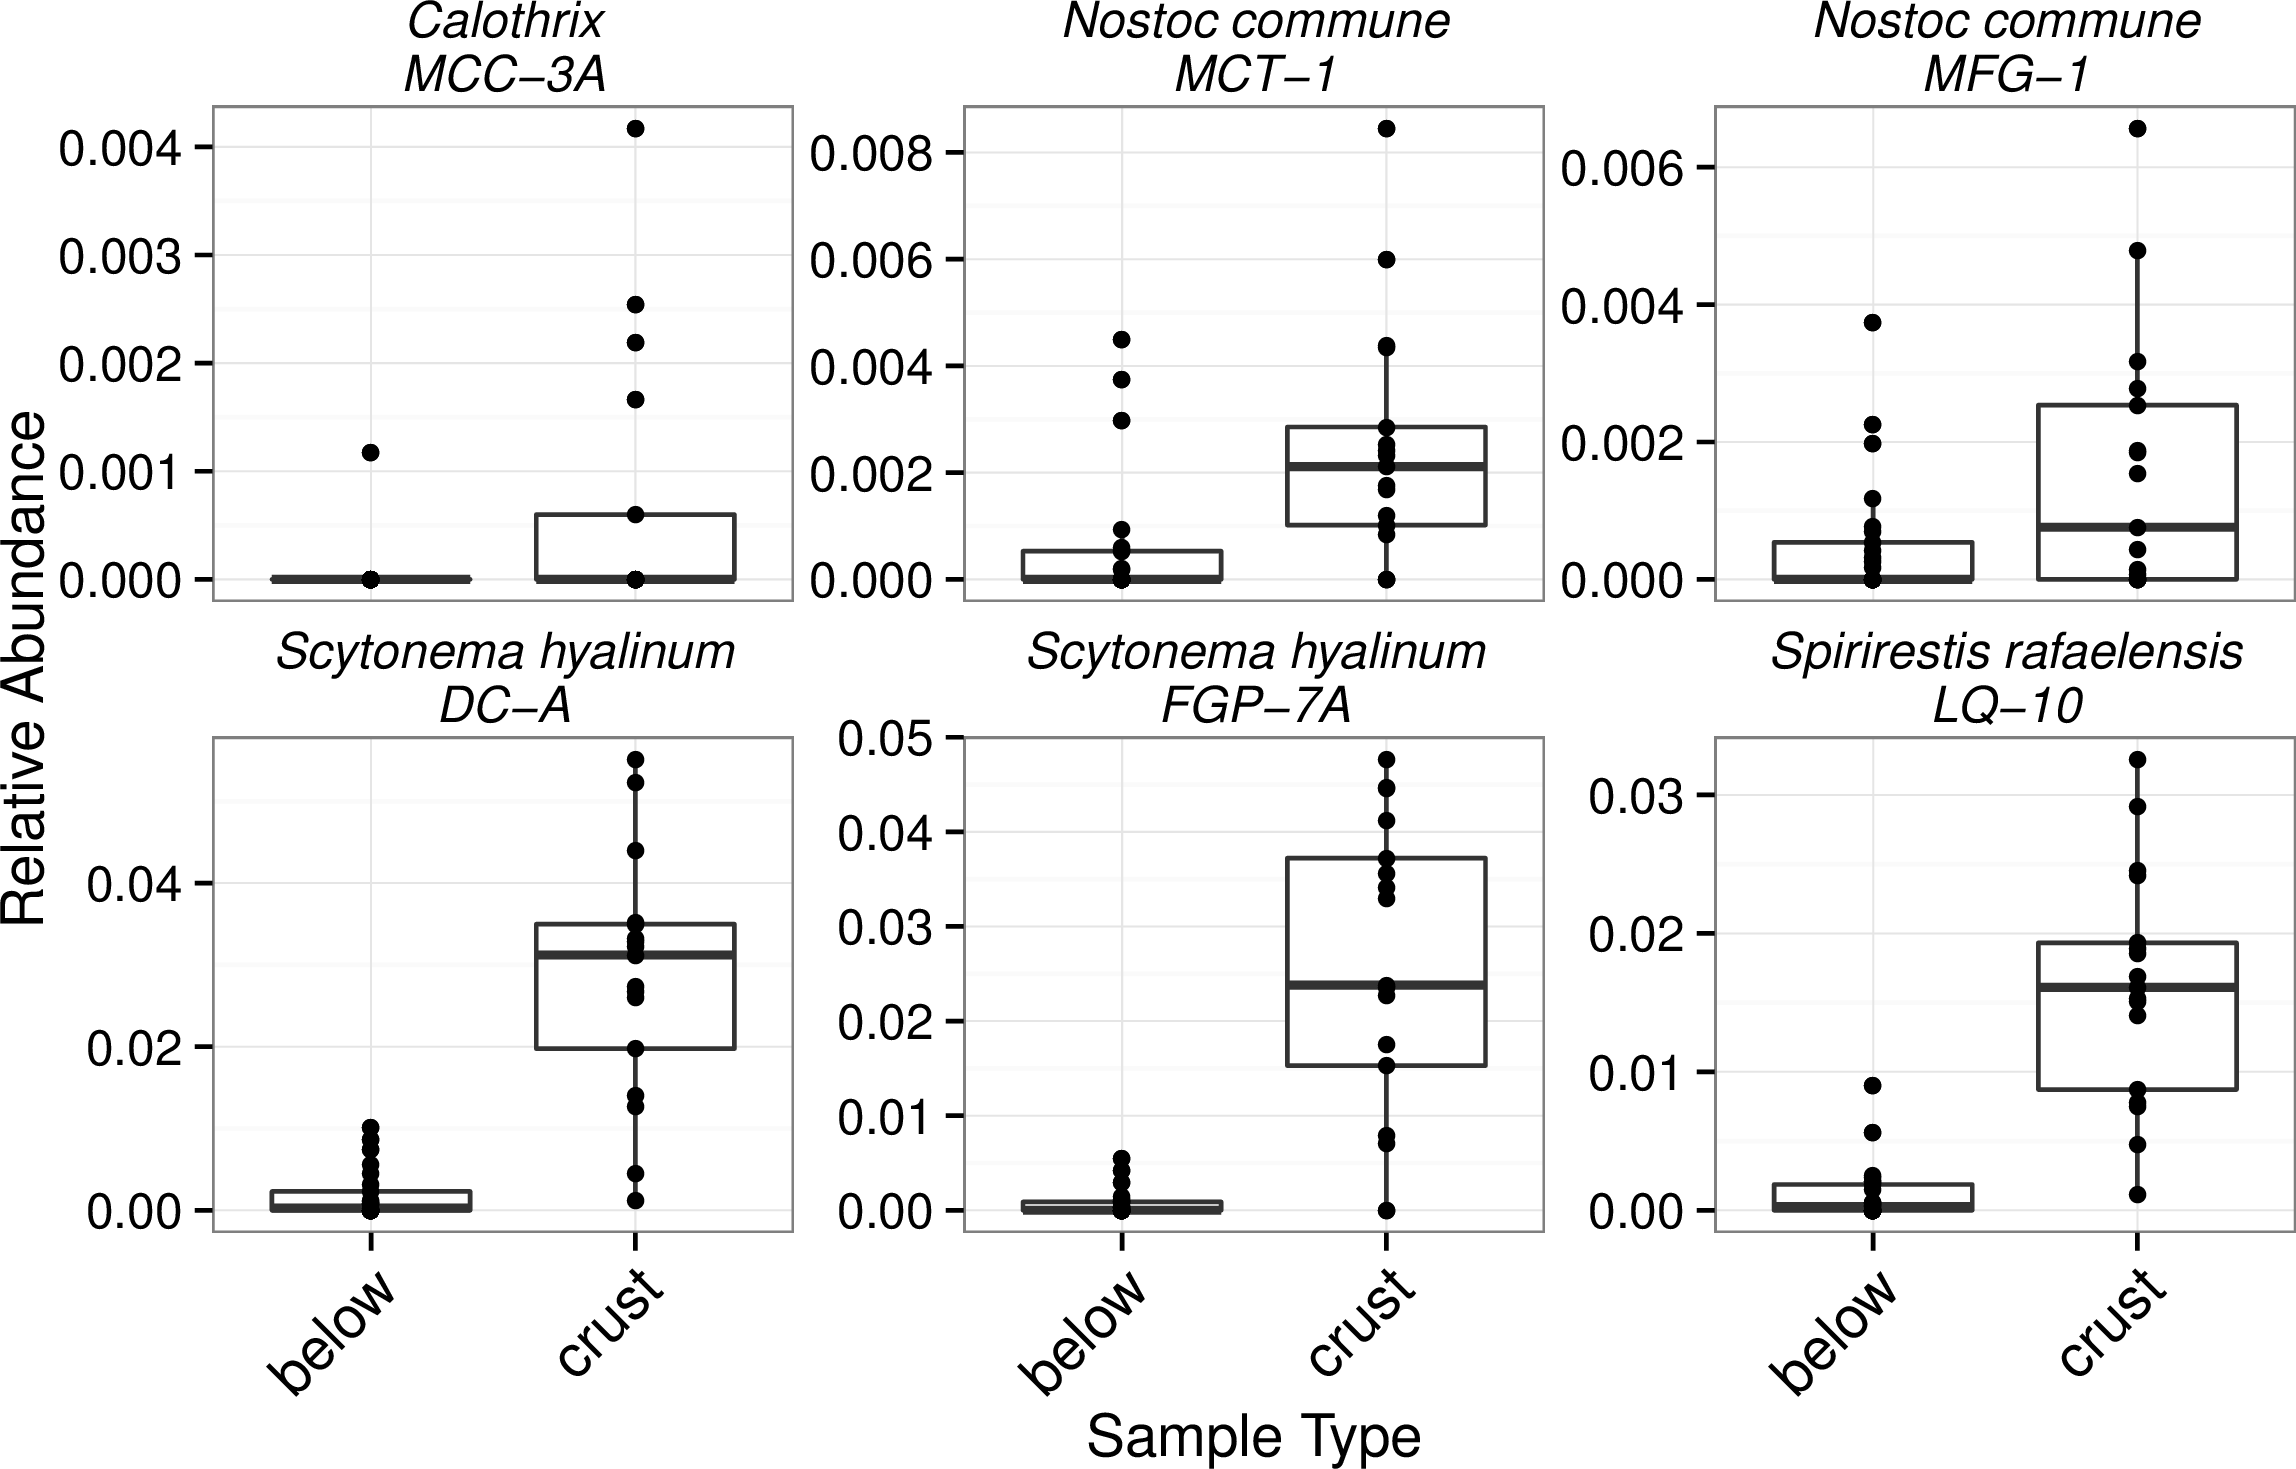
\includegraphics[width=1.0\textwidth]{figures/het_cyano_steven2013/het_cyano_steven2013.png}
  \caption{Relative abundance of selected heterocystous cyanobacterial OTUs with centroids from sequences described in \citet{Yeager} (see methods for selection criteria) in \citet{Steven_2013} data set.}
  \label{fig:het_steven}
\end{figure}

\begin{figure}[h!]
  \centering
    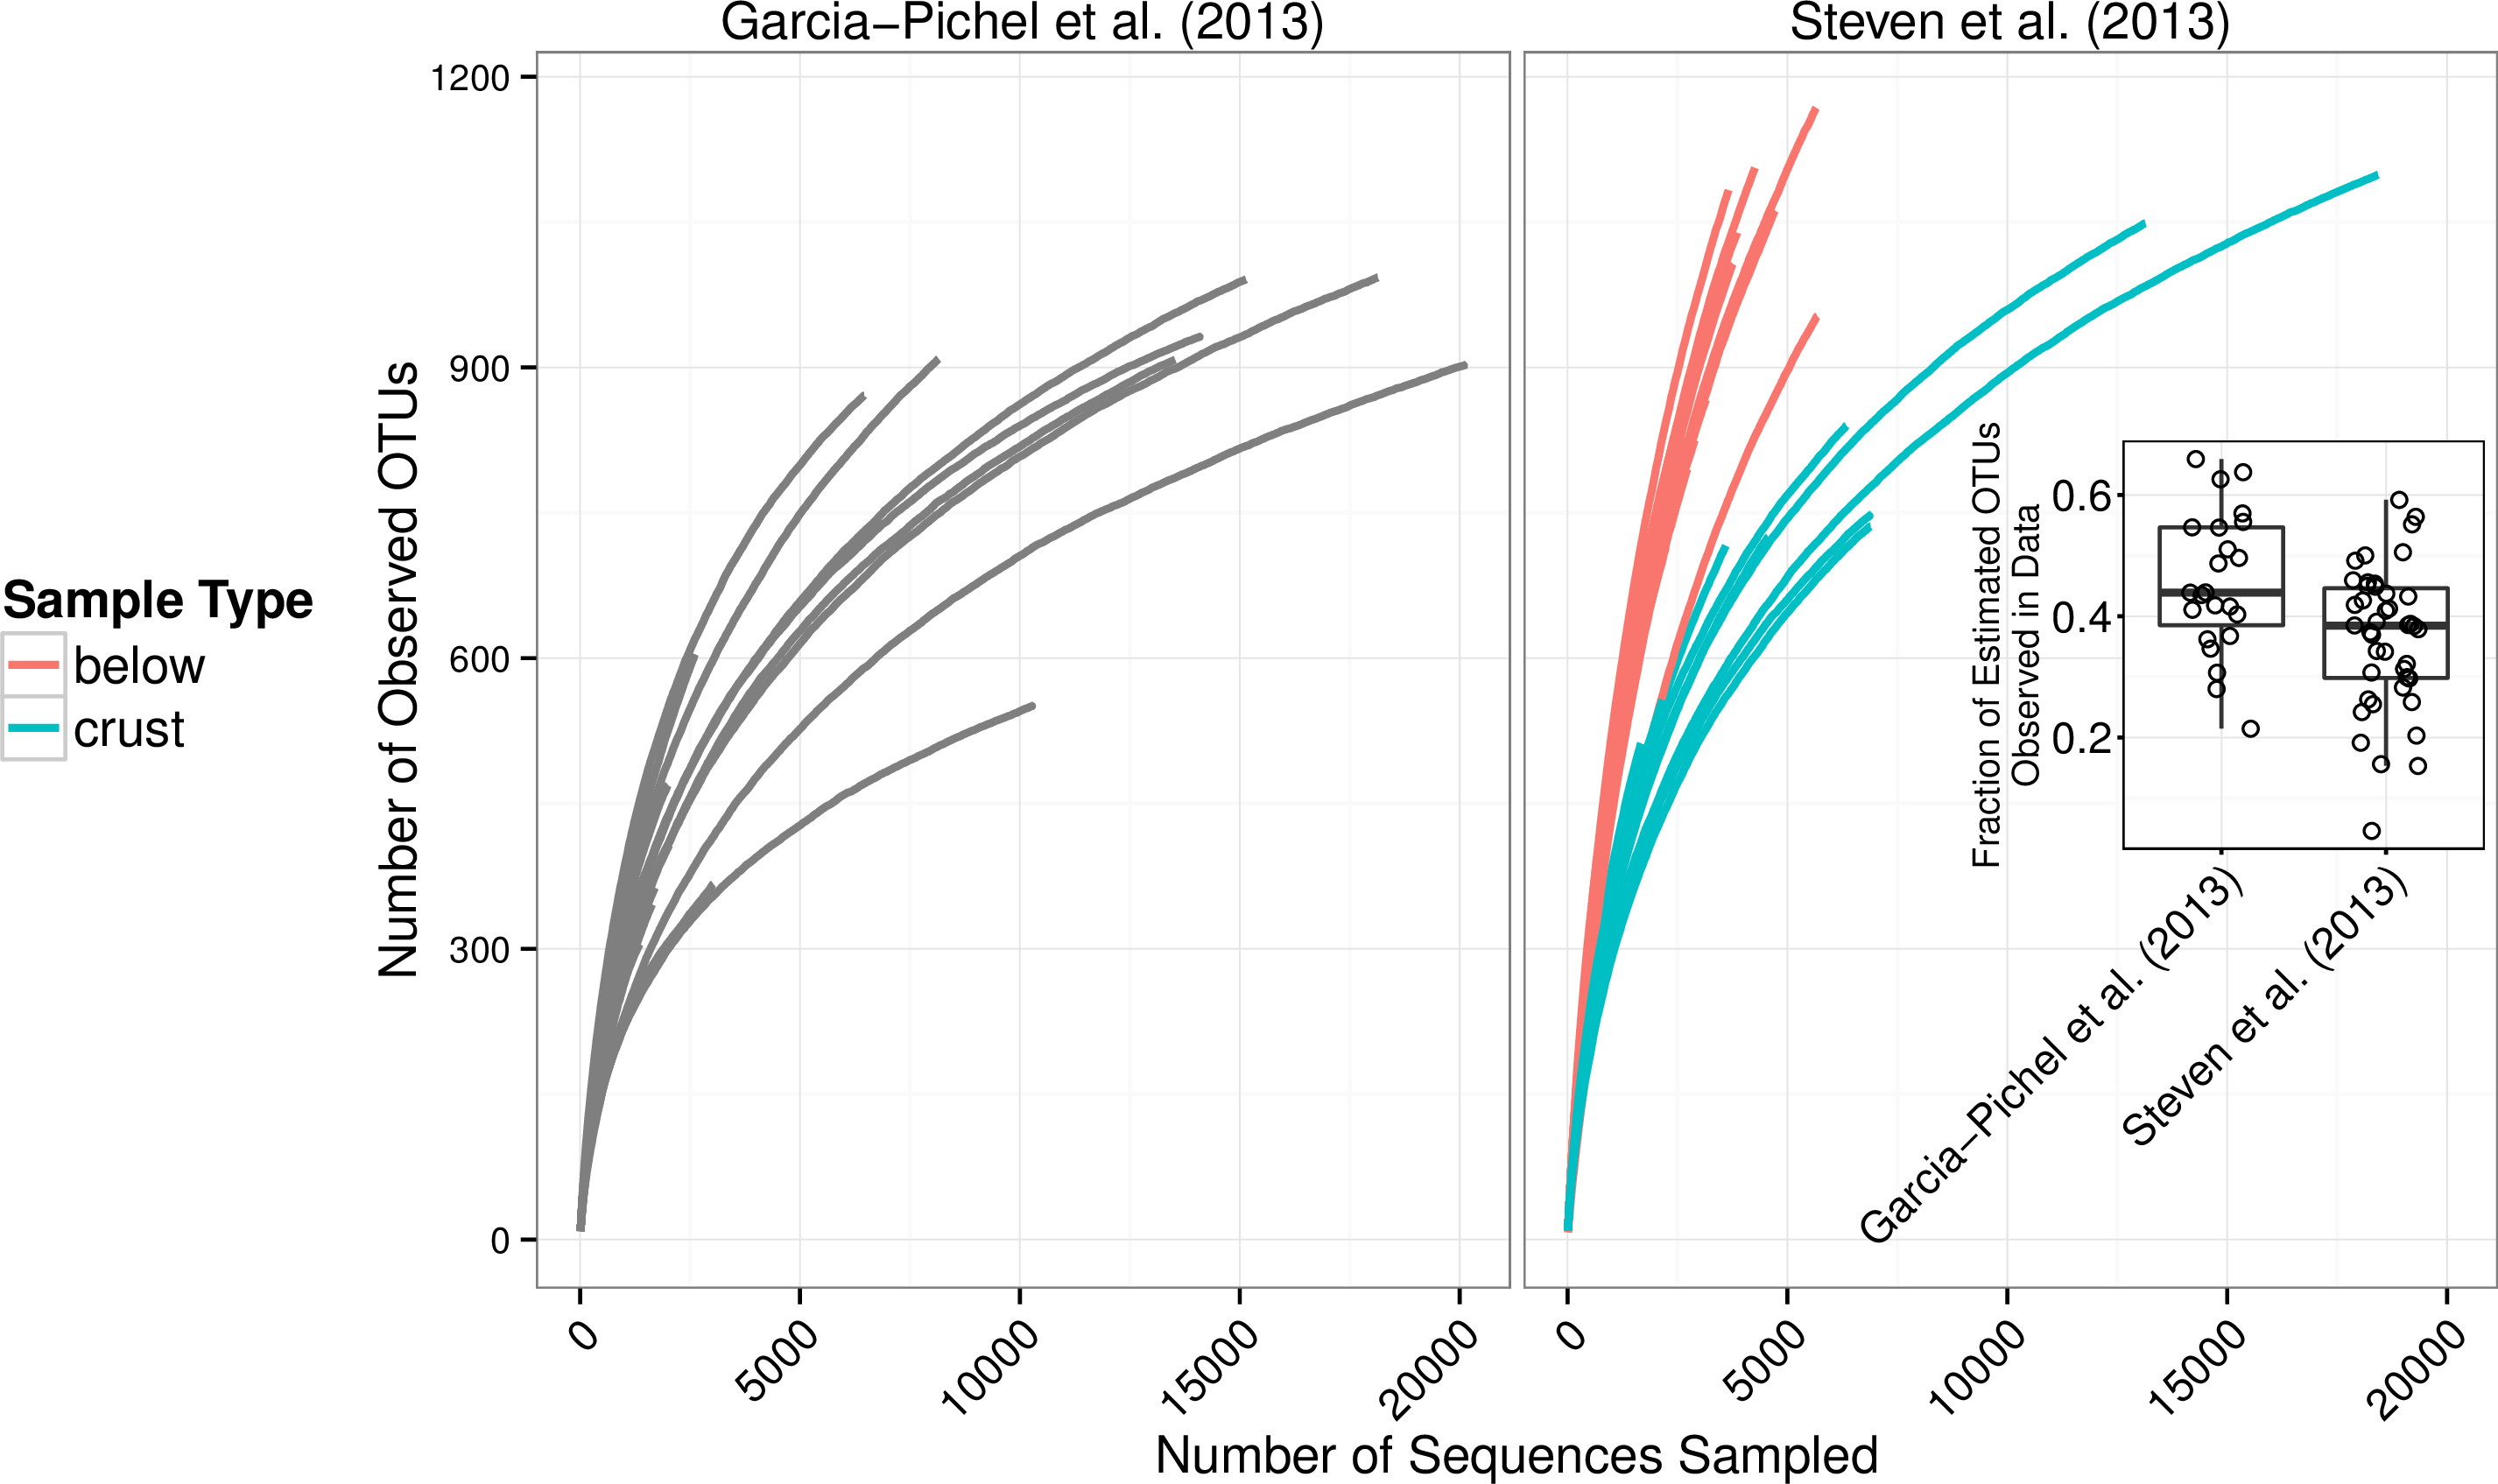
\includegraphics[width=1.0\textwidth]{figures/rarefacation_curves1/raref_and_boxplot.png}
  \caption{Rarefaction curves for all samples presented by \citet{Garcia_Pichel_2013} and \citet{Steven_2013}. Inset is boxplot of estimated sampling effort for all samples in \citet{Garcia_Pichel_2013} and \citet{Steven_2013} (number of observed OTUs divided by number of CatchAll \cite{BUNGE_2010} estimated total OTUs)}
  \label{fig:rarefaction}
\end{figure}

\begin{figure}[h!]
  \centering
    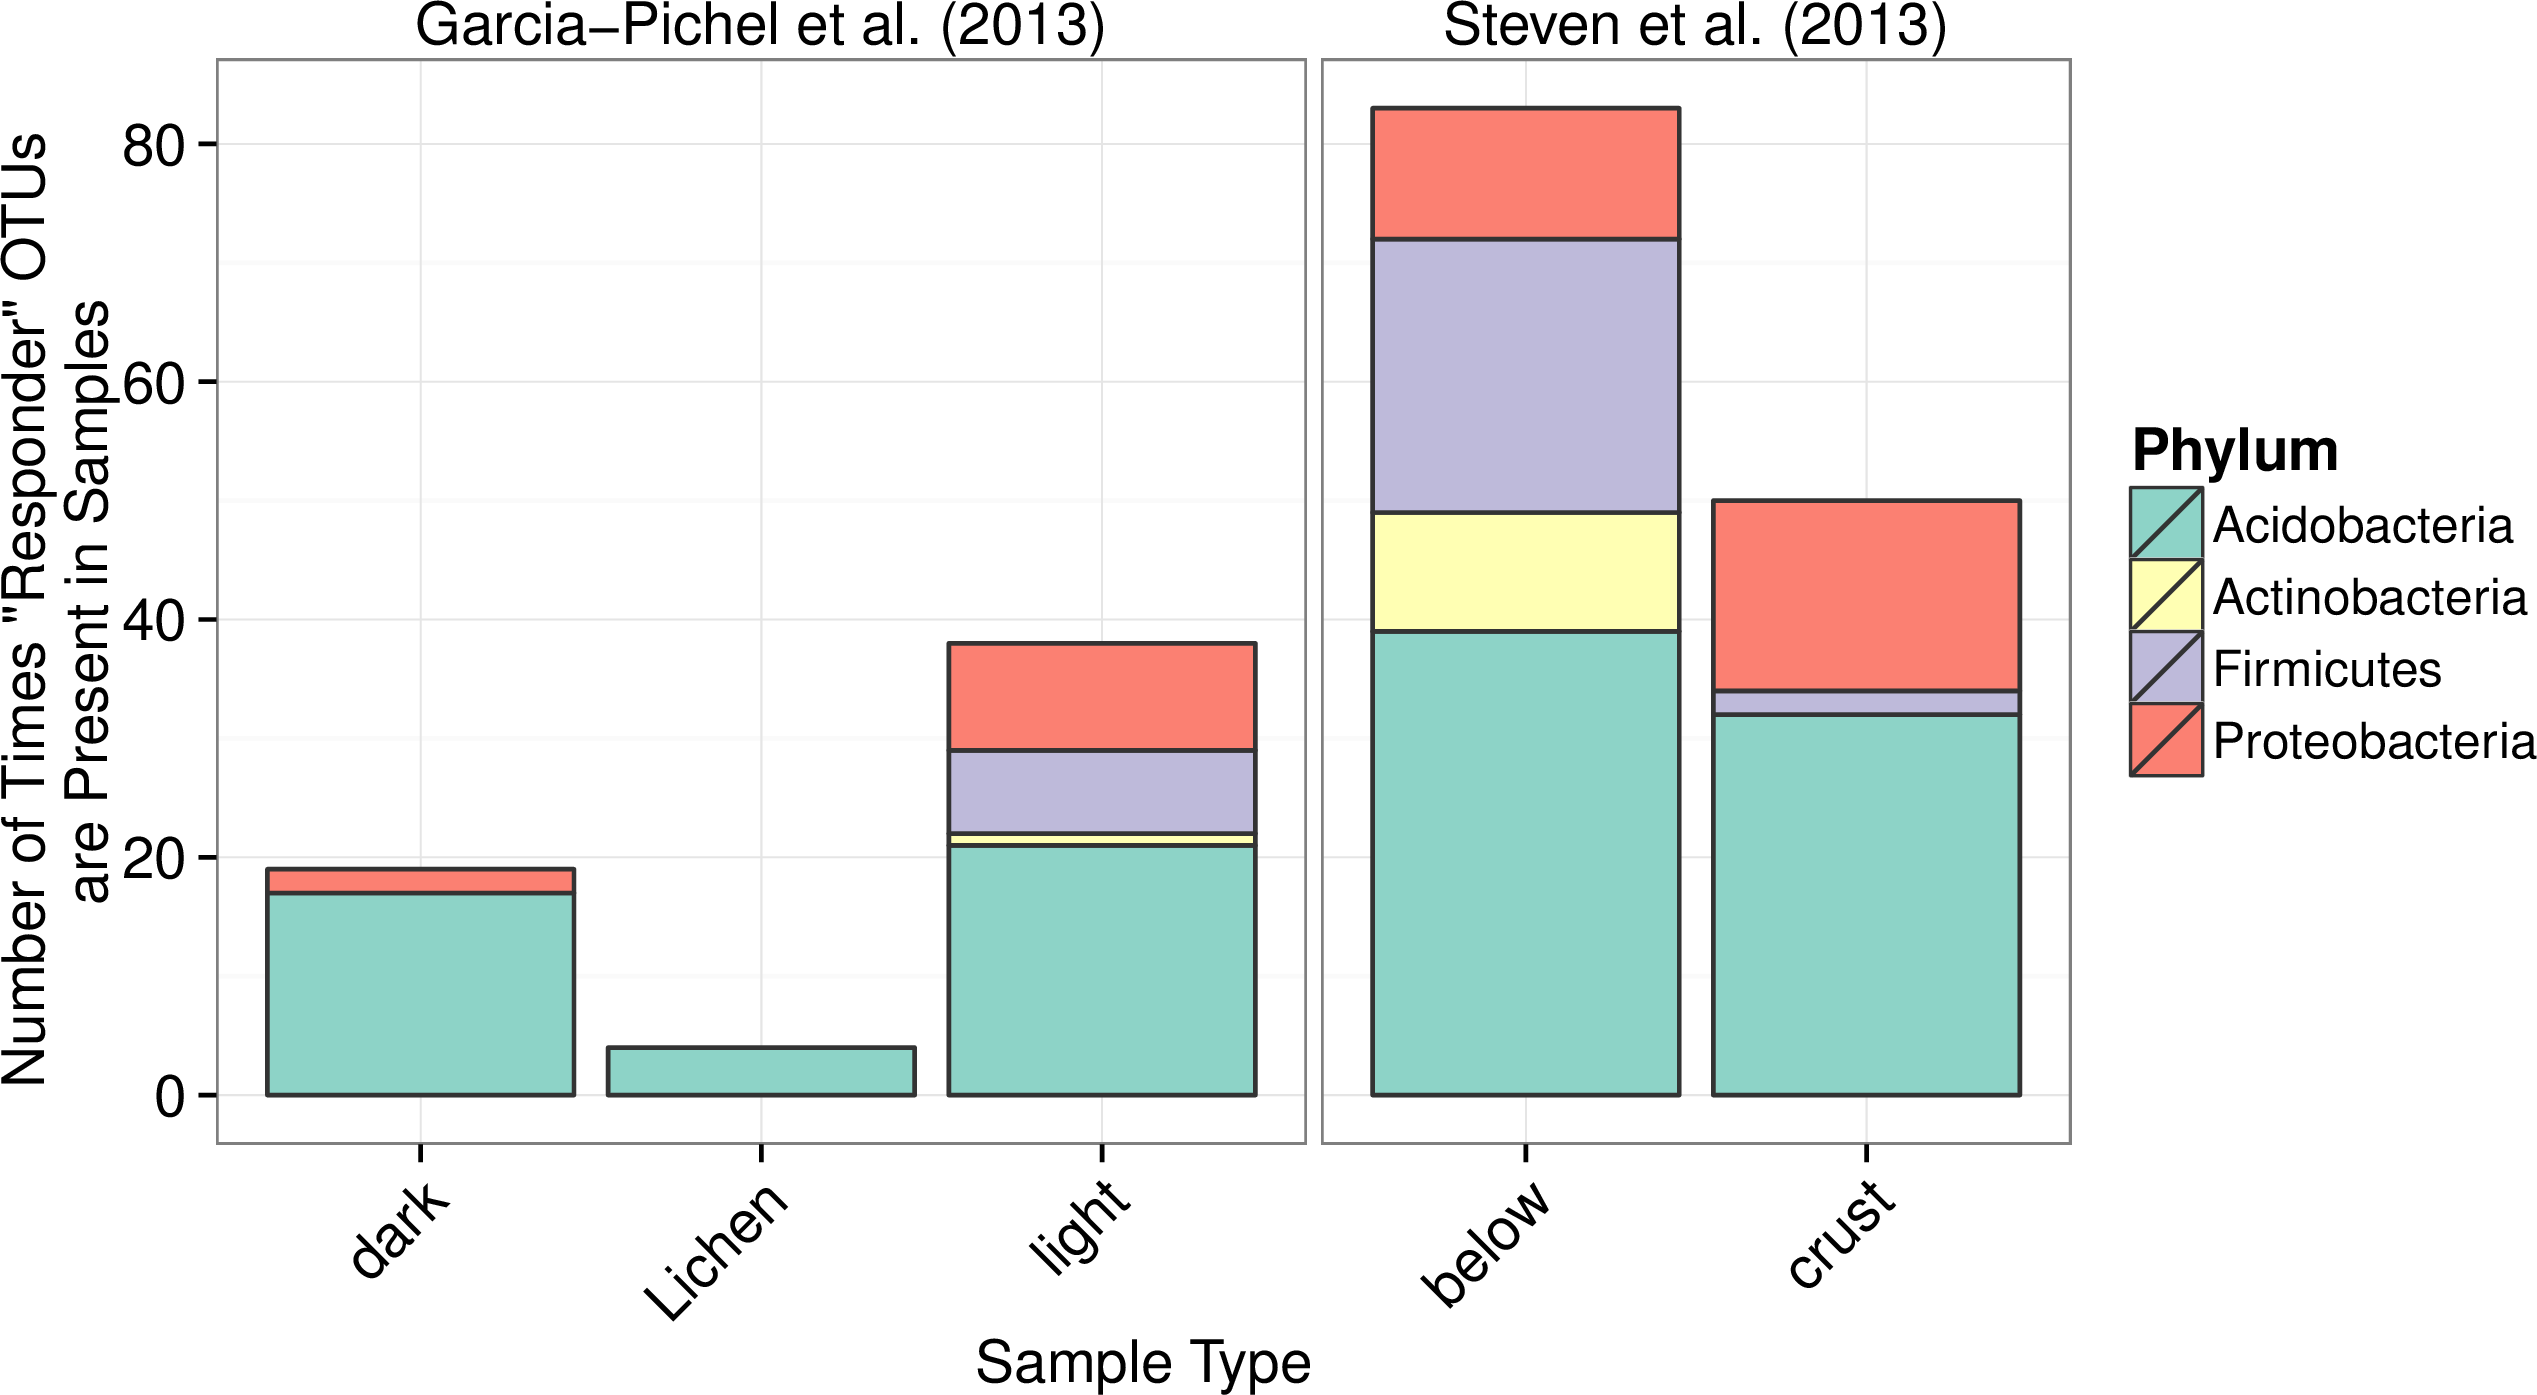
\includegraphics[width=1.0\textwidth]{figures/rspndr_dist/rspndr_dist.png}
  \caption{Counts of "responder" OTU occurrences in samples from \citet{Steven_2013} and \citet{Garcia_Pichel_2013}. \citet{Steven_2013} collected BSC samples (25 samples total) and samples from soil beneath BSC (17 samples total, "below" column in figure). \citet{Garcia_Pichel_2013} collected samples from "dark" (9 samples total) and "light" (12 samples total) crusts in addition to "lichen" (2 samples total) dominated crusts.}
  \label{fig:rspndr_dist}
\end{figure}

\begin{figure}[h!]
  \centering
    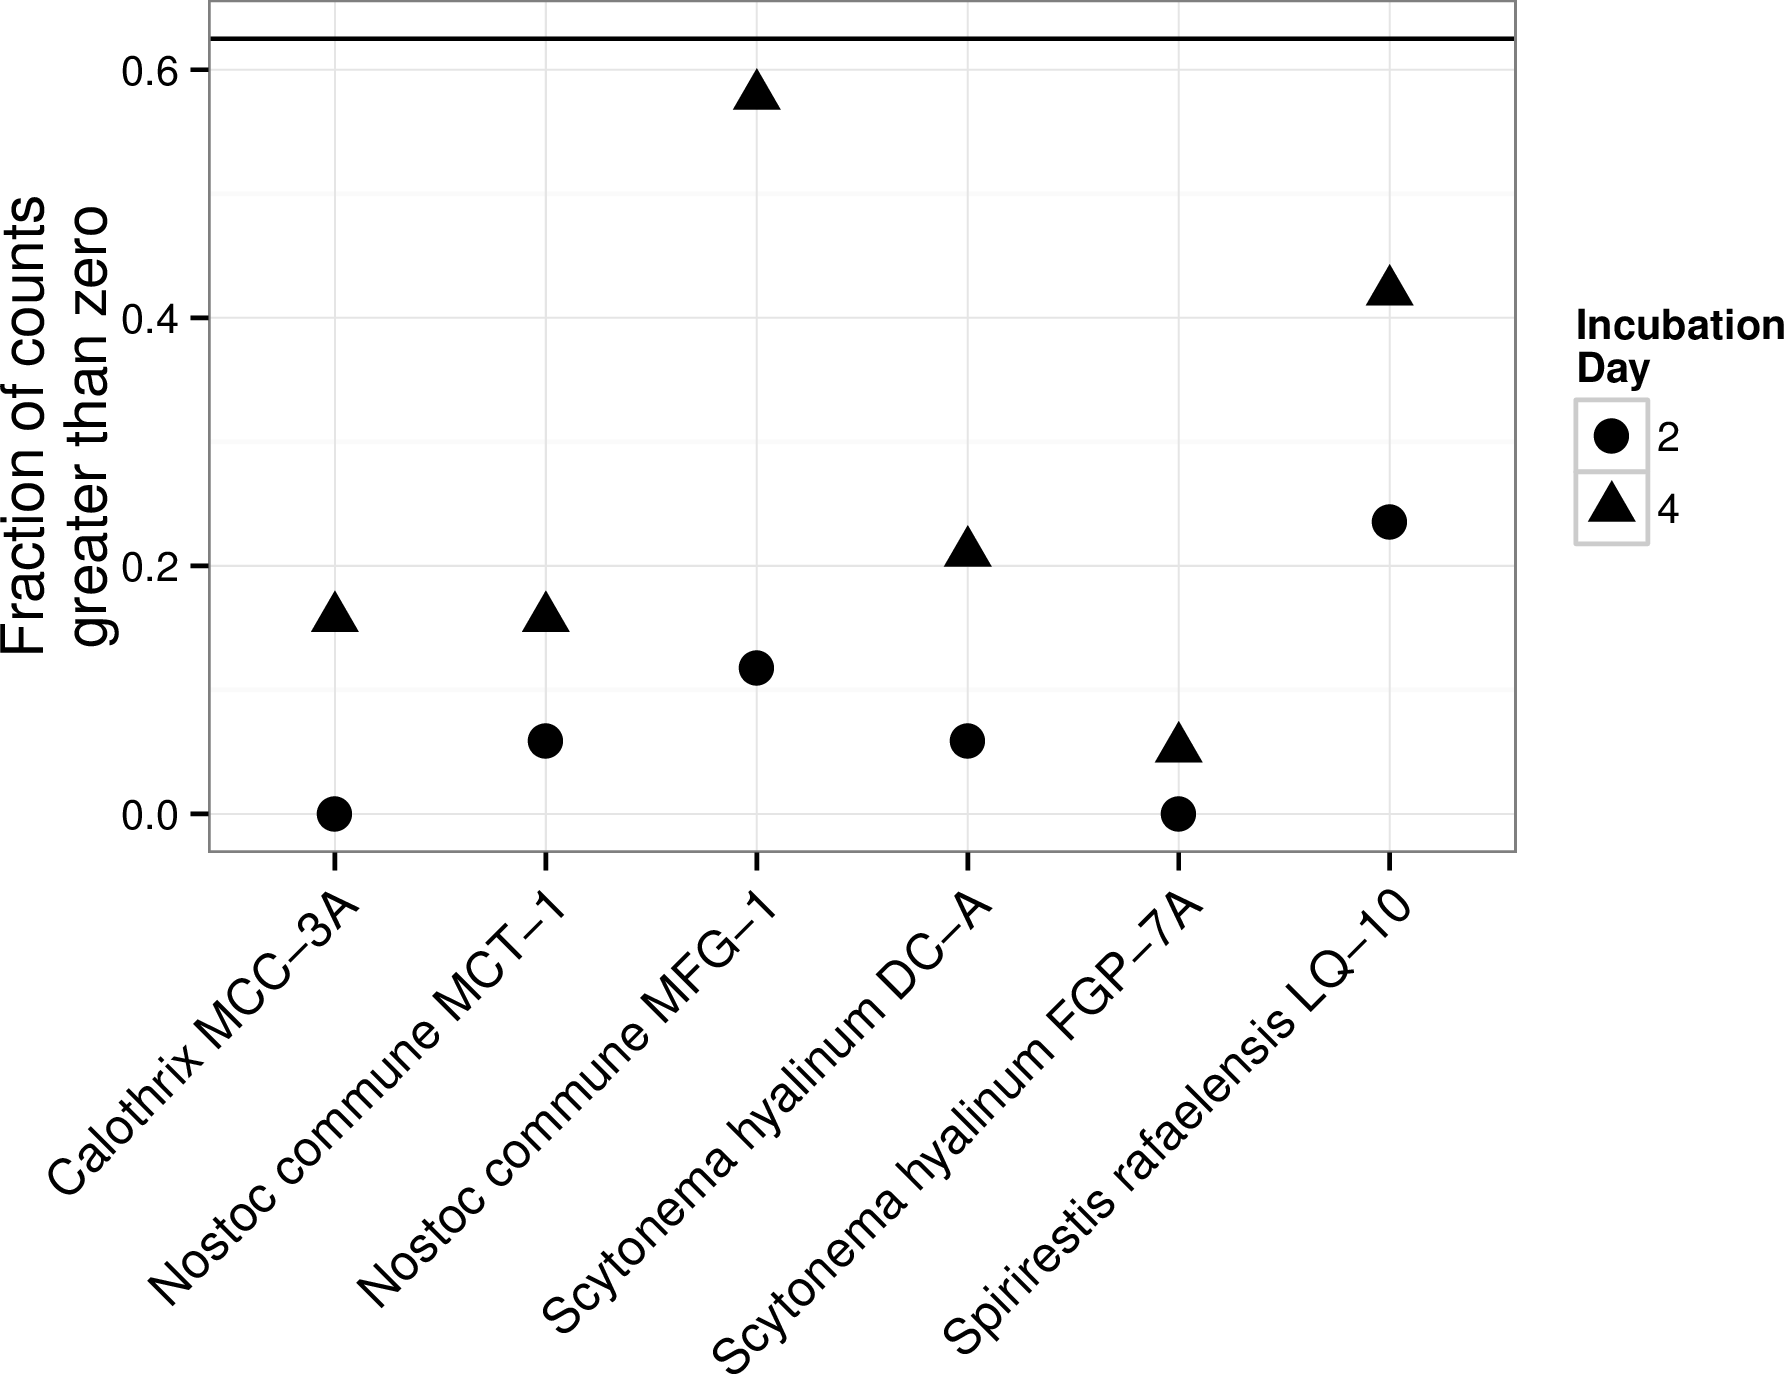
\includegraphics[width=1.0\textwidth]{figures/het_sparsity/het_sparsity.png}
  \caption{Relative abundance of selected heterocystous cyanobacterial OTUs with centroids from sequences described in \citet{Yeager} (see methods for selection criteria) in \citet{Steven_2013} data set.}
  \label{fig:het_sparsity}
\end{figure}

\begin{figure}[h!]
  \centering
    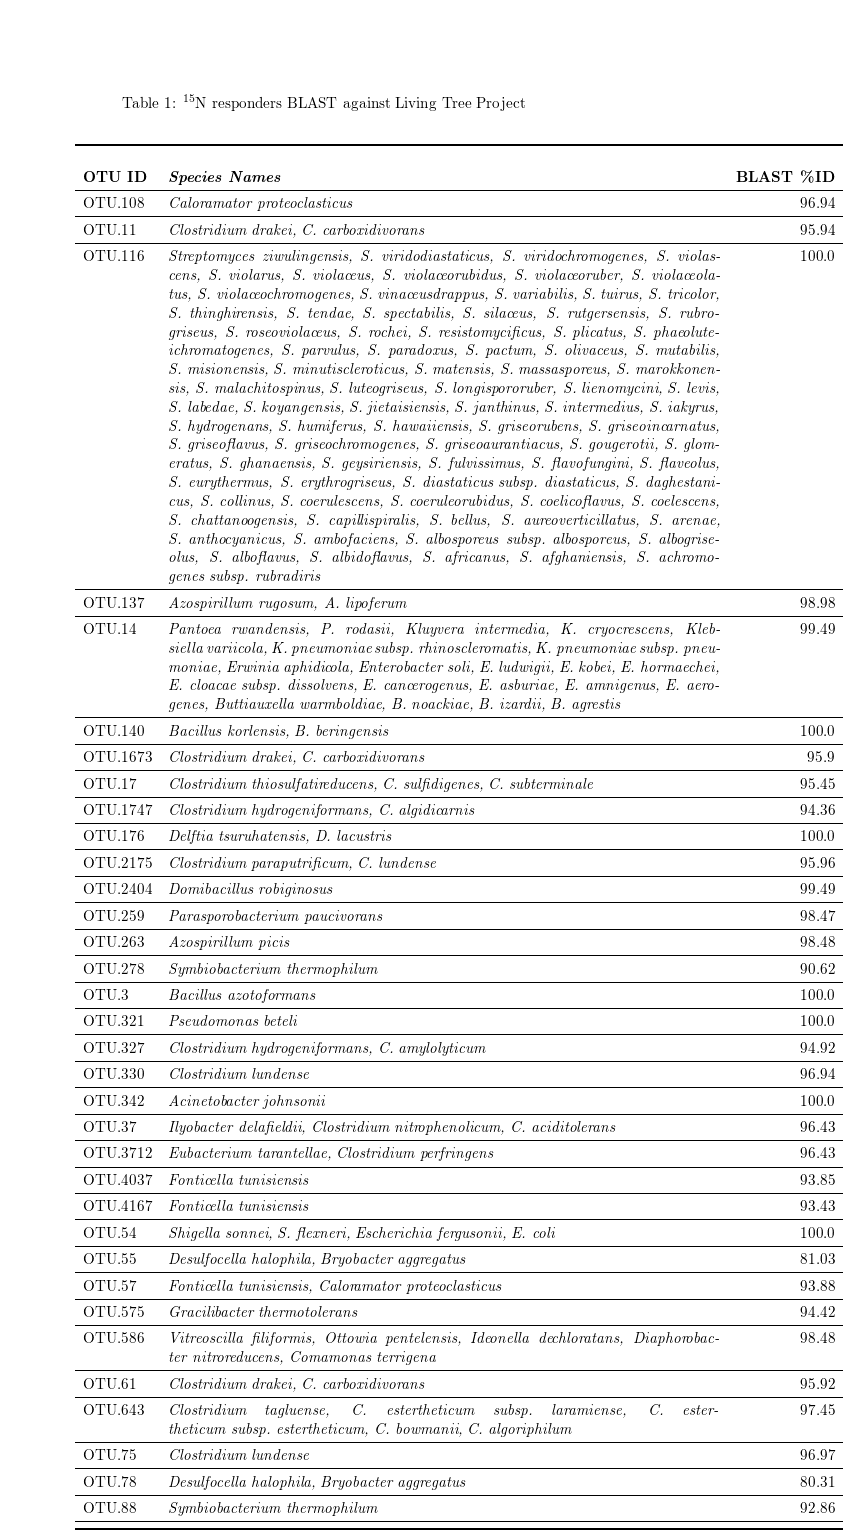
\includegraphics[width=1.0\textwidth]{figures/LTP_blast_table/LTP_blast_table.png}
  \caption{Replace this text with your caption}
  \label{tab:LTP_blast}
\end{figure}

\begin{figure}[h!]
  \centering
    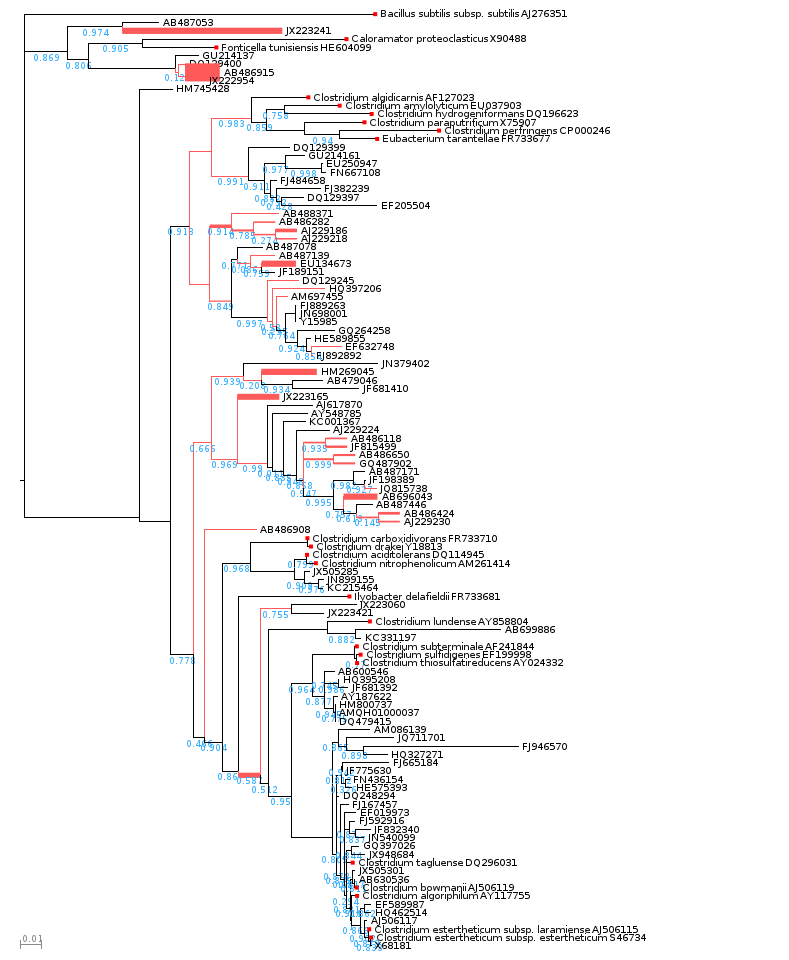
\includegraphics[width=1.0\textwidth]{figures/clost.tree/clost_tree.png}
  \caption{See methods for selection criteria for sequences in backbone tree. Edge width is proportional to number of short putative \textit{Clostridiaceae} diazotroph sequences placed at that position. Placement of short sequences can be spread across multiple edges \cite{Matsen_2010}. Reference sequences from cultivars have boxes at tips and full species names. Tips with only accession annotations are from environmental reference sequences.}
  \label{fig:clost_tree}
\end{figure}
